\documentclass{article}

\usepackage{upquote,graphicx,amsmath,natbib}

\title{On the treatment of discordant detrital zircon U--Pb data}

\author{Pieter Vermeesch\\ Department of Earth Sciences, University
  College London, Gower Street, London WC1E 6BT}

\begin{document}

\maketitle

\begin{abstract}
  Zircon U--Pb geochronology is a staple of crustal evolution studies
  and sedimentary provenance analysis. Constructing (detrital) U--Pb
  age spectra is straightforward for concordant
  \textsuperscript{206}Pb/\textsuperscript{238}U- and
  \textsuperscript{207}Pb/\textsuperscript{206}Pb-compositions.  But
  unfortunately, many U--Pb datasets contain a significant proportion
  of discordant analyses. This paper investigates two decisions that
  must be made when analysing such discordant U--Pb data.

  First, the analyst must choose whether to use the
  \textsuperscript{206}Pb/\textsuperscript{238}U- or the
  \textsuperscript{207}Pb/\textsuperscript{206}Pb-date. The
  \textsuperscript{206}Pb/\textsuperscript{238}U-method is more
  precise for young samples, whereas the
  \textsuperscript{207}Pb/\textsuperscript{206}Pb-method is better
  suited for old samples. However there is no agreement which `cutoff'
  should be used to switch between the two. This subjective decision
  can be avoided by using single grain concordia ages. These represent
  a kind of weighted mean between the
  \textsuperscript{206}Pb/\textsuperscript{238}U- and
  \textsuperscript{207}Pb/\textsuperscript{206}Pb-methods, which
  offers better precision than either of the latter two methods.

  A second subjective decision is how to define the discordance cutoff
  between `good' and `bad' data. Discordance is usually defined as (1)
  the relative age difference between the
  \textsuperscript{206}Pb/\textsuperscript{238}U and
  \textsuperscript{207}Pb/\textsuperscript{206}Pb dates.  However,
  this paper shows that several other definitions are possible as
  well, including (2) the absolute age difference; (3) the common-Pb
  fraction according to the Stacey-Kramers mantle evolution model; (4)
  the p-value of concordance; (5) the perpendicular logratio (or
  `Aitchison') distance to the concordia line; and (6) the logratio
  distance to the maximum likelihood composition on the concordia
  line.

  Applying these six discordance filters to a 70,869-grain dataset of
  zircon U--Pb compositions reveals that: (i) the relative age
  discordance filter tends to suppress the young age components in
  U--Pb age spectra, whilst inflating the older age components; (ii)
  the Stacey-Kramers discordance filter is more likely to reject old
  grains and less likely to reject young ones; (iii) the p-value based
  discordance filter has the undesirable effect of biasing the results
  towards the least precise measurements; (iv) the logratio-based
  discordance filters are most strict for Proterozoic grains, and more
  lenient for Phanerozoic and Archaean age components; (v) of all the
  methods, the logratio distance to the concordia composition produces
  the best results, in the sense that it produces age spectra that
  most closely match those of the unfiltered data: it sharpens age
  spectra but does not change their shape. The popular relative age
  definition fares the worst according to this criterion.  All the
  methods presented in this paper have been implemented in the
  \texttt{IsoplotR} toolbox for geochronology.
\end{abstract}

%\copyrightstatement{TEXT} %% This section is optional and can be used for copyright transfers.


\section{Introduction}  %% \introduction[modified heading if necessary]
\label{sec:intro}

The U--Pb method consists of two paired decay systems, in which two
isotopes of the same radioactive parent (\textsuperscript{238}U and
\textsuperscript{235}U) decay to two isotopes of the same radiogenic
daughter (\textsuperscript{206}Pb and \textsuperscript{207}Pb,
respectively). This paired decay system provides a powerful internal
consistency check for the method, which is absent from other
chronometers. By `double dating' samples with the
\textsuperscript{206}Pb/\textsuperscript{238}U and
\textsuperscript{207}Pb/\textsuperscript{235}U methods (or,
equivalently, the \textsuperscript{206}Pb/\textsuperscript{238}U and
\textsuperscript{207}Pb/\textsuperscript{206}Pb-methods) it is
possible to verify whether the isotopic system is free of primary or
secondary disturbances. The most reliable age constraints are obtained
from samples whose \textsuperscript{206}Pb/\textsuperscript{238}U,
\textsuperscript{207}Pb/\textsuperscript{235}U and
\textsuperscript{207}Pb/\textsuperscript{206}Pb ages are statistically
indistinguishable from each other. U--Pb compositions that fulfil this
requirement are `concordant'. Those that fail to meet it are
`discordant'.

Discordance can be caused by a number of mechanisms, including: (a)
the presence of non-radiogenic (`common') lead; (b) initial
disequilibrium between the short-lived nuclides of the
\textsuperscript{238}U--\textsuperscript{206}Pb and
\textsuperscript{235}U--\textsuperscript{207}Pb decay chains; (c)
partial loss of radiogenic lead during high grade metamorphism; and
(d) mixing of different age domains during micro-analysis
\citep{schoene2014}. These complicating effects can often be diagnosed
and remediated when multiple cogenetic crystals are available from the
same sample. If the aliquots form an isochron (or `discordia') line in
U--Pb isotope space, then this line can be used to recover robust
chronologies from discordant data \citep{ludwig1998}.

Unfortunately, this procedure is rarely or never possible for detrital
samples, in which crystals of datable minerals are not guaranteed to
be cogenetic.  Without a universal mechanism to identify the cause of
U--Pb discordance and remove its effects, detrital geochronologists
have no choice but to accept some discordant analyses and somehow
incorporate them into their age spectra.  There exists a lack of
consensus among the detrital zircon geochronology community on how to
do this.  Two outstanding questions are:

\begin{enumerate}
\item Which age estimate to use? It is widely recognised that
  \textsuperscript{206}Pb/\textsuperscript{238}U age estimates offer
  the optimal accuracy and precision at the young end of the age
  spectrum, whereas the
  \textsuperscript{207}Pb/\textsuperscript{206}Pb method is better
  suited for older samples. However the cutoff between the two clocks
  varies between studies, with values ranging from 800~Ma to 1.5~Ga
  \citep{gehrels2011,spencer2016}.
\item How to quantify discordance?  Most studies define discordance as
  the relative age difference between the
  \textsuperscript{206}Pb/\textsuperscript{238}U and
  \textsuperscript{207}Pb/\textsuperscript{206}Pb ages, but some
  advocate the use of statistical hypothesis tests and p-values to
  quantify discordance \citep{spencer2016}. And even when a
  discordance definition has been agreed upon, there are many ways to
  choose the discordance cutoff. For example, the relative age
  discordance threshold may vary between 10\% and 30\%
  \citep{gehrels2011}.
\end{enumerate}

This paper addresses both of these issues. Section~\ref{sec:whichage}
advocates the use of single-grain concordia ages \citep{ludwig1998} as
a way to avoid the arbitrary cutoff between the
\textsuperscript{206}Pb/\textsuperscript{238}U and
\textsuperscript{207}Pb/\textsuperscript{206}Pb methods. Although
previous workers have argued for the use of single-grain concordia
ages before \citep[see][for a recent example]{zimmermann2018}, this
study uses a semi-analytical model, rather than purely empirical
arguments, to demonstrate the superior precision of this hybrid
chronometer.

Section~\ref{sec:discordance1} compares and contrasts existing
discordance filters based on age disparity and p-values. It shows that
the relative age definition strongly favours older samples over young
ones, and that the p-value definition, which has gained popularity in
recent years, hurts both the accuracy and precision of detrital
geochronology. The age disparity and p-value definitions are heuristic
by nature and are not based on firm statistical or geological
arguments.  Although they are the two most popular definitions of
discordance in use today, they are by no means the only two possible
options.

Section~\ref{sec:discordance2} addresses the inherent biases of the
existing discordance definitions by proposing three new definitions,
which are based directly on U--Pb compositions rather than on the ages
calculated therefrom. The first new definition assumes that the
discordance is caused by the presence of common lead. The other two
new definitions treat U--Pb discordance as a compositional data
problem \citep[\textit{sensu}][]{aitchison1986}.  Isotope ratios are
strictly positive quantities and log-contrasts are the `natural' way
to quantify `distances' between them.  Section~\ref{sec:discordance2}
introduces two logratio definitions of discordance, ignoring and
accounting for analytical uncertainty, respectively.

Although the new definitions are arguably more attractive than the old
ones from a theoretical point of view, this does not guarantee that
they produce more sensible results. To test their performance on real
data, Section~\ref{sec:application} applies the discordance filters to
a compilation of zircon U--Pb data. Although the true age distribution
of this dataset is unknowable, the results suggest that the logratio
based discordance filters produce the most accurate, and most easily
interpretable results. The relative age definition fares the worst.

\section{Which age to choose?}\label{sec:whichage}

\begin{figure}[t]
  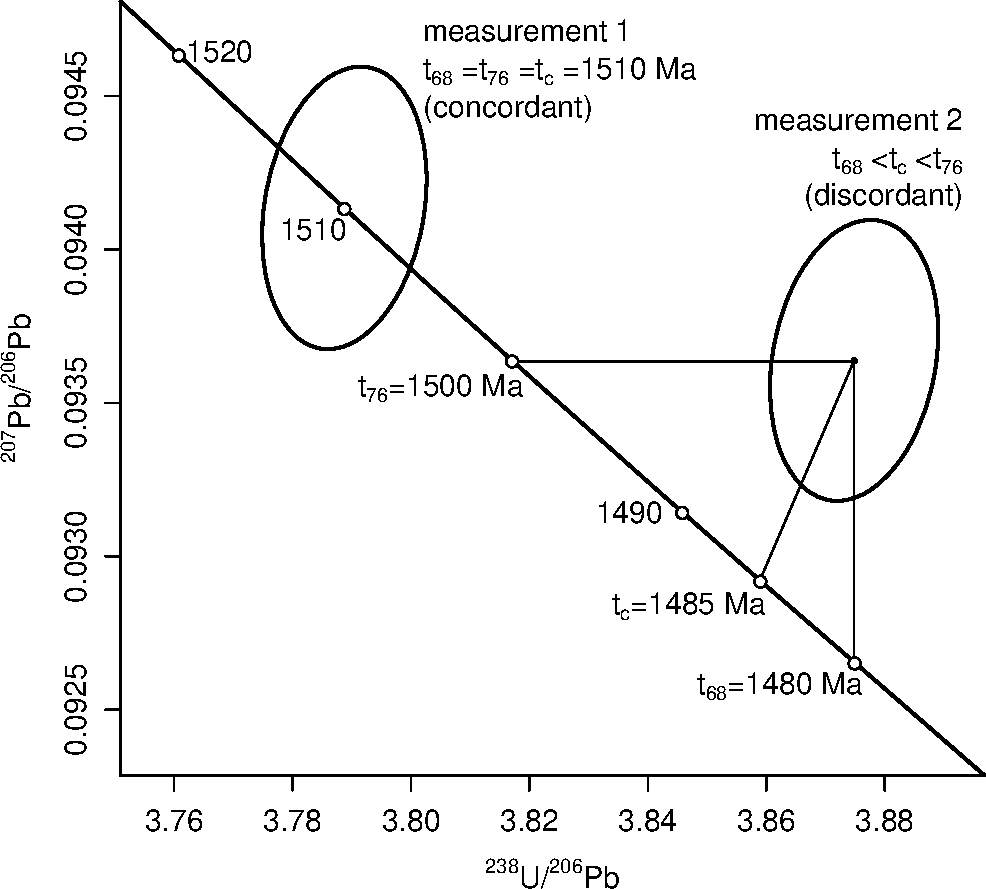
\includegraphics[width=8.3cm]{TW1500.pdf}
  \caption{Illustrative Tera-Wasserburg concordia diagram with a
    concordant and discordant measurement. $t_{68}$ marks the
    \textsuperscript{206}Pb/\textsuperscript{238}U age, $t_{76}$ the
    \textsuperscript{207}Pb/\textsuperscript{206}Pb age, and $t_{c}$
    the concordia age. Measurement~1 is concordant because its
    estimates for $t_{68}$, $t_{76}$ and $t_{c}$ are
    identical. Measurement~2 is discordant because the three estimates
    disagree. The concordia age is the most likely age given the
    analytical uncertainties. It falls between the other two age
    estimates, and offers the best analytical precision of the
    three.}
  \label{fig:concordia}
\end{figure}

The U--Pb method is based on three separate chronometers:
\textsuperscript{206}Pb/\textsuperscript{238}U,
\textsuperscript{207}Pb/\textsuperscript{235}U and
\textsuperscript{207}Pb/\textsuperscript{206}Pb. The half-life of
\textsuperscript{235}U is more than six times shorter than that of
\textsuperscript{238}U, and \textsuperscript{235}U is more than 100
times less abundant than \textsuperscript{238}U. For these two
reasons, little \textsuperscript{207}Pb has been produced during the
last billion years of Earth history compared to
\textsuperscript{206}Pb. Consequently, the
\textsuperscript{207}Pb/\textsuperscript{235}U and
\textsuperscript{207}Pb/\textsuperscript{206}Pb methods are less
precise than the \textsuperscript{206}Pb/\textsuperscript{238}U method
during the Phanerozoic and Neoproterozoic.

However, during earlier stages of Earth's history,
\textsuperscript{235}U was significantly more abundant than it is
today. The \textsuperscript{238}U/\textsuperscript{235}U ratio was
$\sim$60 at 1Ga, $\sim$26 at 2Ga, $\sim$11 at 3Ga, and $\sim$5 at 4Ga.
Due to the greater abundance of \textsuperscript{235}U in this past,
and because it decays much faster than \textsuperscript{238}U, the
precision of the \textsuperscript{207}Pb/\textsuperscript{235}U and
\textsuperscript{207}Pb/\textsuperscript{206}Pb clocks exceeds that of
the \textsuperscript{206}Pb/\textsuperscript{238}U method during the
Palaeoproterozoic and Archaean. The gradual shift in sensitivity
between the two chronometers is visible in the slope of a
Tera-Wasserburg concordia line, which is steep at old ages (high
\textsuperscript{207}Pb/\textsuperscript{206}Pb gradient w.r.t. time)
and shallow at young ages (low
\textsuperscript{238}U/\textsuperscript{206}Pb gradient
w.r.t. time).

Most published detrital zircon U--Pb studies switch from
\textsuperscript{206}Pb/\textsuperscript{238}U to
\textsuperscript{207}Pb/\textsuperscript{206}Pb at some point during
the Proterozoic. Unfortunately there are two problems with such a
switch. First, it requires the selection of a discrete discordance
cutoff between the two methods. If this cutoff differs between two
studies (which it often does), then this complicates the
intercomparison of their respective age spectra. Second, the sudden
switch between the \textsuperscript{206}Pb/\textsuperscript{238}U and
\textsuperscript{207}Pb/\textsuperscript{206}Pb clocks is often marked
by a discrete step in the age spectrum \citep{puetz2018}. This step is
entirely artificial and obscures any geologically significant events
that might occur around the same time.

Both of these problems can be solved by using `hybrid' concordia ages
instead of `pure' \textsuperscript{206}Pb/\textsuperscript{238}U and
\textsuperscript{207}Pb/\textsuperscript{206}Pb ages. Concordia ages
are defined by \citet{ludwig1998} as the `most likely' (in a
statistical sense) U--Pb age given the isotopic ratio composition and
its analytical uncertainty (Figure~\ref{fig:concordia}).  Let $r_{86}$
and $r_{76}$ be the measured
\textsuperscript{238}U/\textsuperscript{206}Pb and
\textsuperscript{207}Pb/\textsuperscript{206}Pb ratios, respectively;
let $\sigma[r_{86}]^2$, $\sigma[r_{76}]^2$ and $\sigma[r_{86},r_{76}]$
be their (co)variances; and let $R_{68}(t) = \exp(\lambda_{238}t) -
1$, $R_{75}(t) = \exp(\lambda_{235}t) - 1$, and $R_{58} =
{}^{235}\mbox{U/}^{238}\mbox{U}$.  Then the concordia age $t_c$ is
obtained by numerically minimising the sum of squares $S$\footnote{The
  same calculation can also be performed in Wetherill space, and is
  actually easier there.}:
\begin{equation}
  S = \left[
    \begin{array}{@{}c@{}}
      r_{86} - 1/R_{68}(t_c) \\
      r_{76} - R_{58} R_{75}(t_c)/R_{68}(t_c)
    \end{array}
    \right]^T\left[
    \begin{array}{@{}cc@{}}
      \sigma[r_{86}]^2 & \sigma[r_{86},r_{76}] \\
      \sigma[r_{86},r_{76}] & \sigma[r_{76}]^2
    \end{array}
    \right]^{-1}
  \left[
    \begin{array}{@{}c@{}}
      r_{86} - 1/R_{68}(t_c) \\
      r_{76} - R_{58} R_{75}(t_c)/R_{68}(t_c)
    \end{array}
    \right]
  \label{eq:S}
\end{equation}

The single grain concordia age combines the chronometric power of the
\textsuperscript{206}Pb/\textsuperscript{238}U and
\textsuperscript{207}Pb/\textsuperscript{206}Pb systems. For young
($<$1~Ga) samples, the concordia age is nearly identical to the
\textsuperscript{206}Pb/\textsuperscript{238}U age. For old samples
($>$2~Ga) it approaches the
\textsuperscript{207}Pb/\textsuperscript{206}Pb age. Using concordia
ages removes the need for an arbitrary cutoff between the two
chronometers. An additional advantage is that the concordia age offers
better precision than the
\textsuperscript{206}Pb/\textsuperscript{238}U and the
\textsuperscript{207}Pb/\textsuperscript{206}Pb chronometer (or the
\textsuperscript{207}Pb/\textsuperscript{235}U for that matter).
Figure~\ref{fig:precision} quantifies this effect using a
semi-analytical mass spectrometry simulation whose algorithm is
provided in Appendix~\ref{app:synthetics}.

\begin{figure}[t]
  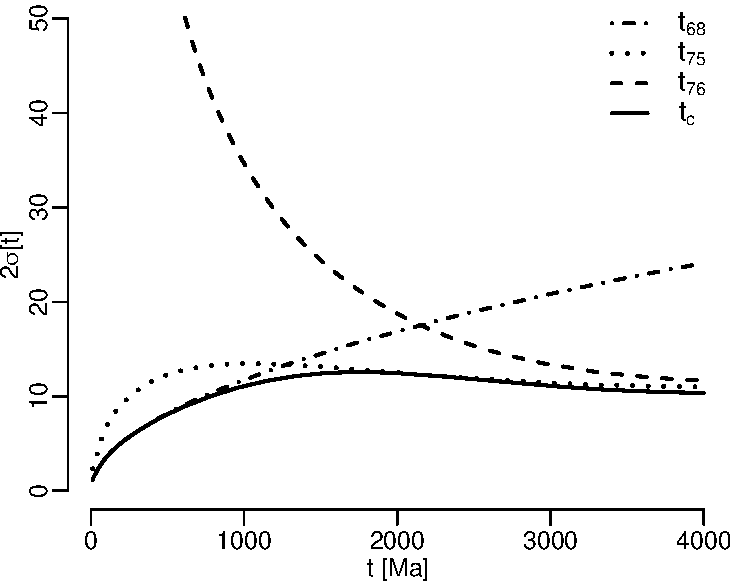
\includegraphics[width=8.3cm]{agerr.pdf}
  \caption{Predicted uncertainties of the
    \textsuperscript{206}Pb/\textsuperscript{238}U ($t_{68}$),
    \textsuperscript{207}Pb/\textsuperscript{235}U ($t_{75}$),
    \textsuperscript{207}Pb/\textsuperscript{206}Pb ($t_{76}$) and
    concordia ($t_c$) ages for a synthetic dataset with a constant
    uranium concentration. Dwell times and detector sensitivities were
    chosen so as to yield results that are similar to those obtained
    from real data. The concordia age (solid line) always offers the
    best precision. See Appendix~\ref{app:synthetics} for further
    details about the calculations behind this figure.}
  \label{fig:precision}
\end{figure}

\section{Discordance filters: old definitions}\label{sec:discordance1}

The most common definition of discordance uses the relative difference
between the \textsuperscript{206}Pb/\textsuperscript{238}U and
\textsuperscript{207}Pb/\textsuperscript{206}Pb age estimate 
\citep{gehrels2011}:
\begin{equation}
  d_r = 1 - t_{68}/t_{76}
  \label{eq:dr}
\end{equation}

However other definitions are possible as well. For example, one could
also define discordance in terms of absolute age differences
\citep{puetz2018}:
\begin{equation}
  d_t = t_{76} - t_{68}
  \label{eq:dt}
\end{equation}

A third option is to define discordance in terms of U--Pb compositions
rather than ages. \citet{spencer2016} advocate using p-values to
assess concordance. In the context of single grain concordia ages, the
p-value is the probability that the sum of squares $S$
(Equation~\ref{eq:S}) exceeds the observed value under a chi-square
distribution with two degrees of freedom:
\begin{equation}
  d_p = \mbox{Prob}\left(s > S | S \sim \chi^2_2
    \right)
  \label{eq:dp}
\end{equation}

Zircon U--Pb data can be filtered by removing all measurements whose
discordance values exceed a certain threshold value. Typical cutoff
values for $d_r$ are 10--30\% \citep{gehrels2011}, whereas $d_p$ is
generally set to 5\% \citep{spencer2016}. Different discordance
criteria produce different U--Pb age spectra. For example, a relative
age cutoff will preferentially remove young grains whereas an absolute
age cutoff is comparatively more likely to remove old grains
(Figure~\ref{fig:agediscordance}).

\begin{figure}[t]
  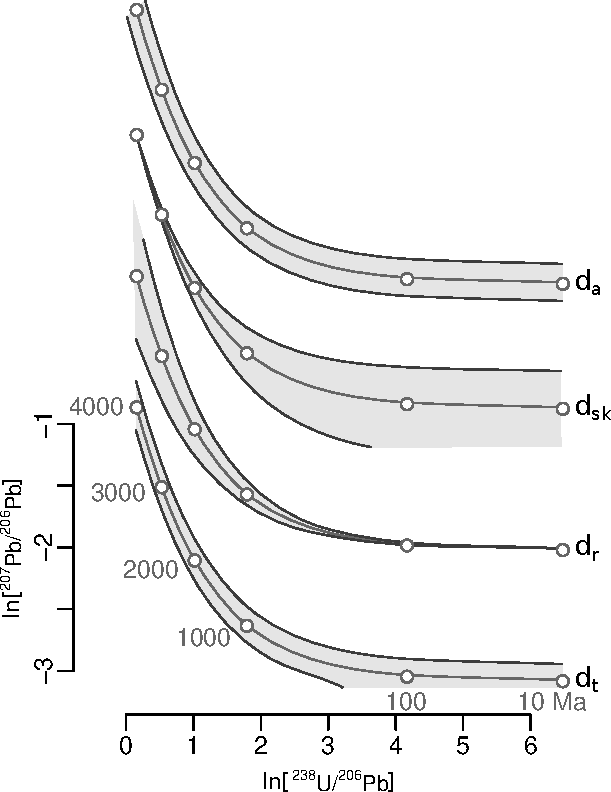
\includegraphics[width=8.3cm]{TW-option-1234.pdf}
  \caption{Discordance cutoffs for four of the six discordance
    definitions discussed in Sections~\ref{sec:discordance1} and
    \ref{sec:discordance2}. The $d_{p}$ and $d_c$ criteria are not
    shown because they depend on the analytical uncertainty of the
    measurements, which may vary between studies. The grey envelopes
    mark cutoff values of $d_r=20\%$ (relative age filter),
    $d_t=300$~Ma (absolute age filter), $d_{sk}=2\%$ (Stacey--Kramers
    filter) and $d_{a}=15\%$ (perpendicular Aitchison distance) on a
    Tera-Wasserburg concordia diagram, which is plotted in logarithmic
    space to provide a more balanced view of the old and young ends of
    the time scale. The $d_{sk}$ and $d_t$ envelopes are truncated
    where they cross over into physically impossible negative isotope
    ratio space.}
  \label{fig:agediscordance}
\end{figure}

The p-value definition affects grains differently depending on their
analytical precision \citep{nemchin2005}. For example, consider a
1.5~Ga zircon that is $d_r=1\%$ discordant. If this grain were
analysed by LA-ICP-MS with an analytical precision of 2\%, say, then
it would pass the chi-square test and be accepted as being
concordant. However, if that same grain were analysed by TIMS with a
precision of 0.2\%, then the p-value criterion would reject it as
being discordant (Figure~\ref{fig:TIMSvsLAICPMS}). It seems
fundamentally wrong that an imprecise analytical method would be
favoured over a precise one. This is a pertinent problem because
technical innovations are increasing the precision of all analytical
approaches to U--Pb geochronology.  As precision improves, so does the
ability to detect ever small degrees of discordance. Using the p-value
criterion, there may come a time when no zircon passes this filter.

A final argument against the p-value discordance criterion is that it
biases against old U--Pb ages. This is because old zircon contains
more radiogenic Pb than young zircon does. Therefore the analytical
precision of the isotopic ratio measurements tends to be better for
old grains than it is for young ones. Consequently, the chi-square
test has greater power \citep[\emph{sensu}][]{cohen1992} to reject
them. In conclusion, p-value based discordance filters are
fundamentally flawed. Despite their appeal as `objective' tools for
statistical decision making, formalised hypothesis tests such as
chi-square are rarely useful in geology. For the same reason, the
widely used MSWD \citep[Mean Square of the Weighted
  Deviates,][]{mcintyre1966} statistic (which is just $S$/2 in this
case) should be used with caution. This is because, like p-values,
also MSWD cutoffs punish precise datasets in favour of imprecise
ones. Note that this caveat also goes against the recommendations of
\citet{spencer2016}.

\begin{figure}[t]
  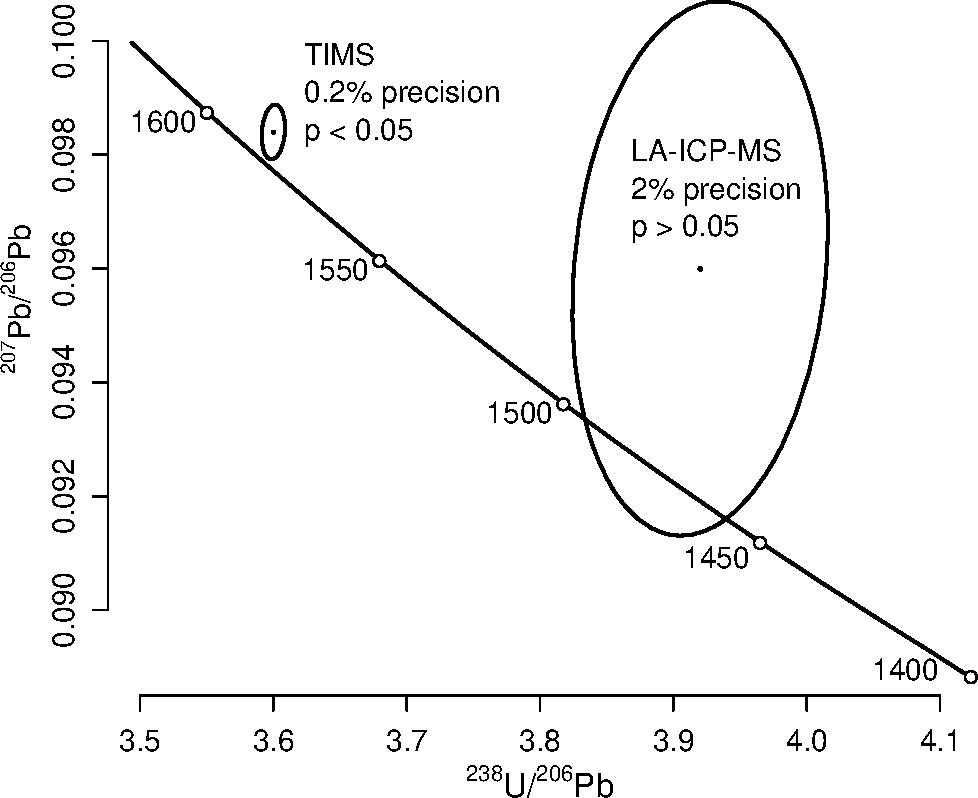
\includegraphics[width=8.3cm]{TIMSvsICPMS.pdf}
  \caption{Application of the flawed p-value discordance criterion
    to two synthetic measurements by TIMS (left) and LA-ICP-MS
    (right).  The precise TIMS measurement is labelled as discordant
    even though it plots closer to the concordia line than the
    imprecise LA-ICP-MS measurement, which is labelled as
    concordant.
  }
  \label{fig:TIMSvsLAICPMS}
\end{figure}

\section{Discordance filters: new definitions}\label{sec:discordance2}

\begin{figure}[t]
  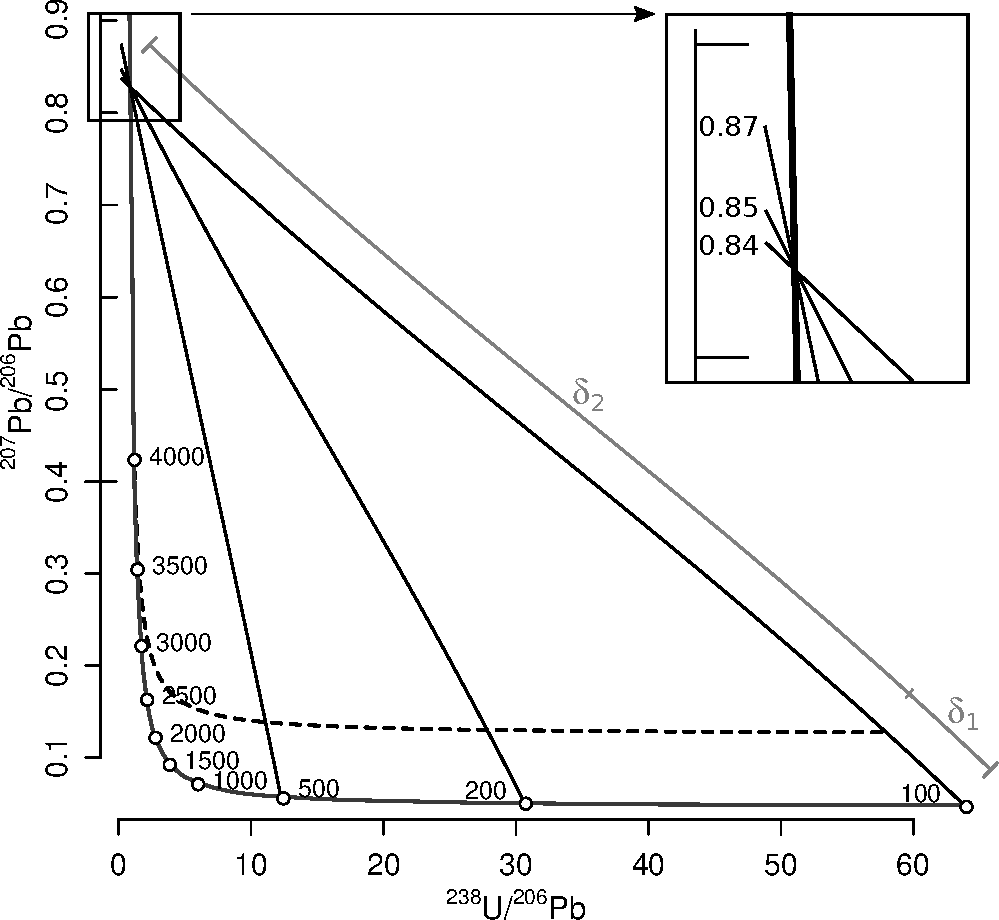
\includegraphics[width=8.3cm]{TW-sk.pdf}
    \caption{Using the \citet{stacey1975} common Pb model as a
      discordance criterion. This criterion assumes that the
      discordance is caused by linear mixing (hence, the linear scale
      of this Tera-Wasserburg plot) between radiogenic Pb
      (intersections of the mixing lines with concordia) and common Pb
      (intersection of the mixing lines with the vertical axis, see
      inset). The dashed line marks the 20\% ($=
      \delta_1/[\delta_1+\delta_2]$) discordance cutoff. This
      discordance filter, which must be applied \emph{before} making
      any actual common Pb correction, is more forgiving for young
      grains than it is for old grains. In this respect, it has the
      opposite effect of the relative age filter shown in
      Figure~\ref{fig:agediscordance}.  }
    \label{fig:SK}
\end{figure}

Section~\ref{sec:discordance1} reviewed three existing discordance
definitions.  This Section will introduce three new ones.  None of the
definitions discussed thus far encode any information about the
geological mechanisms behind the discordance. As explained in
Section~\ref{sec:intro}, common Pb is one of the most likely causes of
discordance. Using a mantle evolution model \citep[e.g.][]{stacey1975}
to approximate the isotopic composition of this common Pb, discordance
can be defined as:
\begin{equation}
  d_{sk} = 1 - r_{86}/r_{86}^\ast
  \label{eq:dsk}
\end{equation}

\noindent where $r_{86}^\ast$ is the
\textsuperscript{238}U/\textsuperscript{206}Pb-ratio of the
intersection between concordia and a straight line connecting the
\textsuperscript{238}U/\textsuperscript{206}Pb--\textsuperscript{207}Pb/\textsuperscript{206}Pb
measurement to the inferred mantle composition (Figure~\ref{fig:SK}).

The common Pb definition of discordance is more forgiving for young
grains than it is for old ones. Importantly, if the discordance is
caused by common Pb, then the
\textsuperscript{206}Pb/\textsuperscript{238}U,
\textsuperscript{207}Pb/\textsuperscript{206}Pb and concordia age
estimates are all positively biased with respect to the true
age. However this bias can be removed by applying a common-Pb
correction \emph{after} the data have been filtered.

Even though Equation~\ref{eq:dsk} is mathematically able to produce
negative discordance values, such values cease to have a geologically
meaningful interpretation, because it is impossible for minerals to
inherit negative amounts of common Pb. Thus it may be sensible to set
a minimum cutoff of $d_{sk}>0$ when using the Stacey-Kramers filter.

Each discordia definition that we have studied thus far is expressed
in different units. For the absolute age definition, degrees of
discordance are expressed in units of time (ranging from 0 to
4.5~Ga). The relative age definition uses fractions of time (ranging
from $-\infty$ to 1). The p-value definition expresses discordance in
terms of probability (ranging from 0 to 1). And the \citet{stacey1975}
definition uses fractions of ratios (ranging from $-\infty$ to
1). None of these scales is particularly intuitive or natural. They
certainly do not match the usual definition of \emph{distance} in the
geographical sense of the word.

To address this issue, it is useful to subject the U--Pb isotopic
ratio data to a logarithmic transformation. So instead of analysing
the data on a conventional Tera-Wasserburg concordia diagram, all
calculations can be done in
ln(\textsuperscript{207}Pb/\textsuperscript{206}Pb) vs.
ln(\textsuperscript{238}U/\textsuperscript{206}Pb) space. The
advantage of this transformation is that it produces values that are
free to range from $-\infty$ to $+\infty$. Within this infinite
dataspace, the Euclidean distance metric can be safely applied.

\begin{figure}
  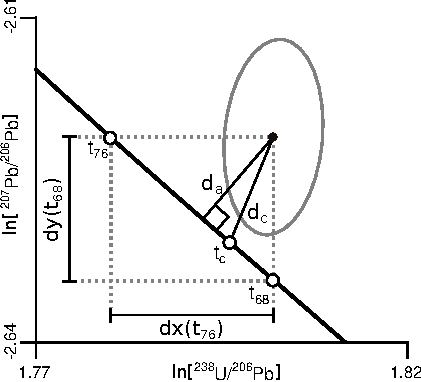
\includegraphics[width=8.3cm]{Aitchison.pdf}
  \caption{Illustration of the two logratio distance definitions of
    discordance. $d_a$ is the perpendicular Aitchison distance from
    the measured logratio to the concordia line. $d_c$ is the
    Aitchison distance measured along a line connecting the measured
    value and the concordia composition.
  }
  \label{fig:aitchison}
\end{figure}

There exists a vast body of statistical literature detailing the
theoretical and practical advantages of logratio analysis. A deeper
discussion of this topic falls outside the scope of this paper, but
the interested reader is referred to \citet{aitchison1986} and
\citet{pawlowsky2015} for further information. The Euclidean distance
between logratios is also known as the `Aitchison distance'.
Discordance can be redefined as the Aitchison distance from the
measured logratios to the concordia line. We introduce two ways to do
so here.  A first option is to simply measure the distance along a
perpendicular line to the concordia curve
(Figure~\ref{fig:aitchison}):
\begin{equation}
  d_{a} = dx(t_{76})
  \sin\!\left(\arctan\!\left[ \frac{dy(t_{68})}{dx(t_{76})} \right]
  \right)
  \label{eq:dperp}
\end{equation}

\noindent where
\begin{equation}
\begin{split}
  dx(t)  = & \ln\!\left[r_{86}\right] + \ln\!\left[R_{68}(t)\right] \\
  \mbox{~and~}
  dy(t) = & \ln\!\left[r_{76}\right] -
  \ln\!\left[R_{58}\frac{R_{75}(t)}{R_{68}(t)}\right]
  \end{split}
\end{equation}

This definition produces a parallel band around the concordia line in
logarithmic Tera-Wasserburg space. In contrast with $d_r$, $d_t$,
$d_{sk}$, the $d_a$ criterion is less strict at both the young and old
extremes of the geological timescale, and more strict during the
Proterozoic Eon, when the U--Pb method is most reliable.

The perpendicular Aitchison distance criterion does not take into
account the analytical precision of the isotopic measurements.  To
address this issue, we can also measure the Aitchison distance along a
line connecting the measured logratio and the maximum likelihood
composition on the concordia line:
\begin{equation}
  d_c = \mbox{sgn}[t_{76}-t_{68}] \sqrt{ dx(t_c)^2 + dy(t_c)^2 }
  \label{eq:da}
\end{equation}

\noindent where sgn[$\ast$] stands for ``the sign of $\ast$'', which
produces positive values for measurements that plot above the
concordia line, and negative values for measurements that plot below
it.

\section{Application to a compilation of zircon U--Pb data}
\label{sec:application}

It is difficult to ascertain the mechanism causing discordance in any
particular zircon grain. Therefore, it is unclear which of the
definitions in Sections~\ref{sec:discordance1} and
\ref{sec:discordance2} is `correct'. All we can do is apply the
methods to real samples and investigate their outcomes. This Section
will apply the discordance filters to a dataset of 70,869 zircon U--Pb
analyses that were acquired by Sensitive High Resolution Ion
Micro-Probe (SHRIMP) mass spectrometery and compiled by Dr. S.
Bodorkos of Geoscience Australia.

The dataset includes 1,665 sedimentary, igneous and metamorphic
samples, mostly from Australia but including some other locations as
well.  The data were acquired by a variety of instruments (including
SHRIMP-1, -2 and -RG) using a range of different reference materials,
and processed on a range of different data reduction software
(including Squid-1, -2 and Prawn/Lead). The data were not subjected to
any common Pb correction or other filters, and were saved in a
Tera-Wasserburg format with zero error correlation between the
\textsuperscript{238}U/\textsuperscript{206}Pb and
\textsuperscript{207}Pb/\textsuperscript{206}Pb ratio uncertainties.

Figure~\ref{fig:KDE} shows the frequency distribution of the complete,
unfiltered dataset as a kernel density estimate. The
\textsuperscript{207}Pb/\textsuperscript{235}U,
\textsuperscript{206}Pb/\textsuperscript{238}U and concordia age
spectra all look similar. However, the
\textsuperscript{207}Pb/\textsuperscript{206}Pb age distribution
deviates from the other three chronometers. It reduces the prominence
of the young age components, and inflates the old end of the age
spectrum.

\begin{figure}[t]
  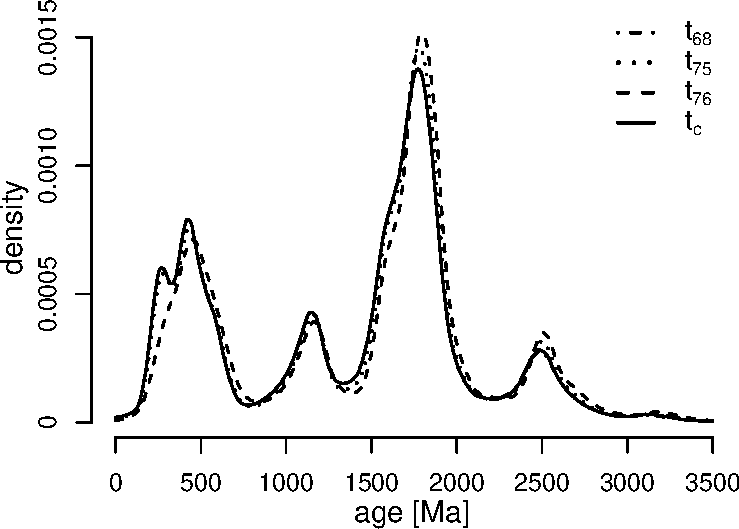
\includegraphics[width=8.3cm]{KDE.pdf}
  \caption{Four superimposed kernel density estimates (KDEs, using a
    50~Myr bandwidth) for 70,869 unfiltered zircon U--Pb dates. The
    \textsuperscript{207}Pb/\textsuperscript{235}U,
    \textsuperscript{206}Pb/\textsuperscript{238}U and concordia age
    spectra are similar.  However the KDE of the
    \textsuperscript{207}Pb/\textsuperscript{206}Pb data stands apart
    from the other three curves. It deviates both at the young end of
    the age spectrum (which it suppresses), and at the old end (which
    it inflates).  }
  \label{fig:KDE}
\end{figure}

Figure~\ref{fig:KDEs} applies five of the six discordance filters to
this database (the p-value filter was omitted for reasons given in
Section~\ref{sec:discordance1}). In order to emphasise the difference
between the discordance definitions whilst treating them on an equal
footing, each of the filters was adjusted until half of the data were
removed. This was achieved by discordance cutoffs of
$-18.6<d_t<46.0$~Myr, $-1.4<d_r<3.66$\%, $-0.11<d_{sk}<0.27$\%,
$-0.78<d_{a}<1.94$\%, and $-0.91<d_c<2.20$\%.

There are noticeable differences between the density estimates.  As
expected from the theoretical considerations laid out in
Sections~\ref{sec:discordance1} and \ref{sec:discordance2}, the
relative age filter greatly suppresses the younger age components
($<1.5$~Ga) relative to the older parts of the age spectrum
($>1.5$~Ga). The \citet{stacey1975} filter has the opposite effect.
It suppresses the Archaean age component by $\sim{50}$\% whilst
further increasing the prominence of the Neoproterozoic and
Phanerozoic modes.

The discordance definitions based on the absolute age difference and
logratio distances have a comparatively minor effect on the shape of
the age spectrum. The change in shape between the age spectrum of the
full (unfiltered) dataset and the age spectra of the filtered datasets
can be visually assessed on quantile-quantile plots and quantified
using the Kolmogorov-Smirnov (KS) statistic \citep{vermeesch2013}.  If
the KS-misfit is taken as a measure of success, then the concordia
distance filter ($d_c$) is the most effective discordance
criterion. It `sharpens' the spectrum without changing the relative
prominence of the modes at 400, 1200, 1800, and 2500~Ma.

\begin{figure*}[t]
  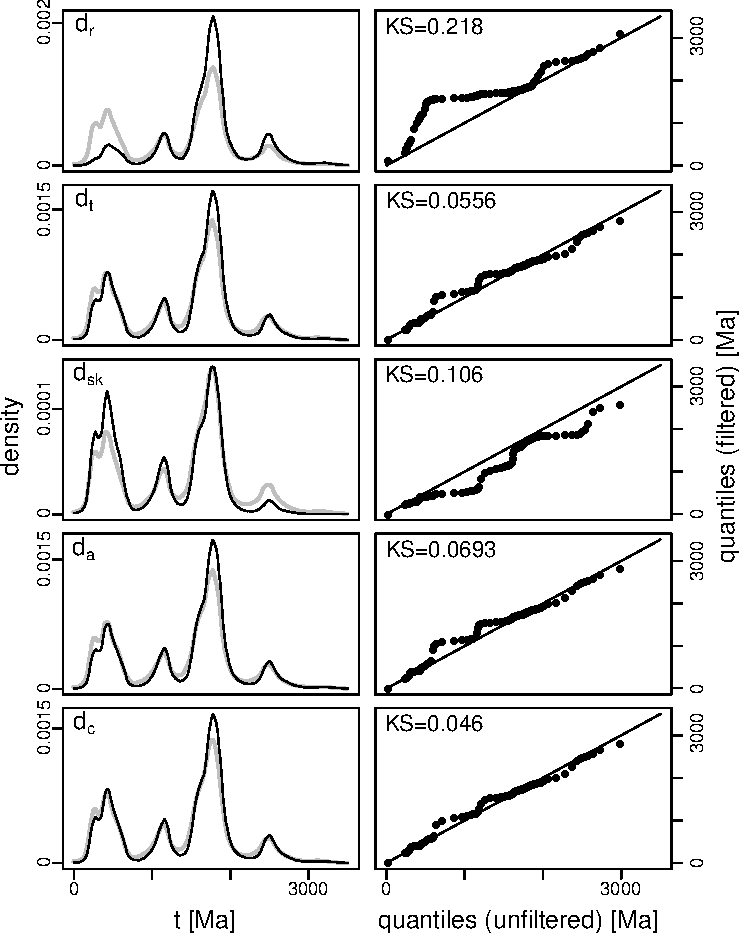
\includegraphics[width=12cm]{KDEs.pdf}
  \caption{Left: filtered U--Pb age spectra for the test data,
    removing the 50\% most discordant grains according to five
    discordance filters reviewed in this paper, shown as a kernel
    density estimate with 50~Myr bandwidth. The complete (unfiltered)
    dataset is shown in grey. Right: quantile-quantile plots comparing
    the filtered and unfiltered datasets. KS = the Kolmogorov-Smirnov
    statistic. The relative age filter ($d_r$) introduces the greatest
    and the concordia distance ($d_c$) the smallest bias,
    respectively.}
  \label{fig:KDEs}
\end{figure*}

Figure~\ref{fig:KDEs} removed 50\% of the data, in order to emphasise
the differences between the discordance filters. In real applications,
less stringent discordance filters are usually applied. As mentioned
in the introduction, most current detrital zircon studies apply a
10\%--30\% relative age cutoff.  Using the test data, we can evaluate
the equivalent values for the $d_t$, $d_{sk}$, $d_a$ and $d_c$
criteria (Table~\ref{tab:conversiontable}). For example, a relative
age filter of 10\% removes the same fraction of the test data as an
absolute age filter with $d_t=97$~Myr, a Stacey-Kramers filter with
$d_{sk}=0.62$\%, a perpendicular Aitchison filter with $d_a=4.1$\%, or
a concordia distance filter with $d_c=4.6$\%.

The p-value discordance filter has been omitted from this comparison
for two reasons. First, the use of this filter is discouraged for
reasons given in Section~\ref{sec:discordance1}. Second, the p-value
cutoffs that are equivalent to any given relative age difference are
highly laboratory dependent, with precise equipment requiring
different $d_p$-cutoffs than imprecise instruments. The other five
discordance filters are more universally applicable. So using a
different set of test data should only make a relatively minor
difference to the values in Table~\ref{tab:conversiontable}.

\begin{table}
  \begin{tabular}{c|cccc}
    $d_r$ & $d_t$ & $d_{sk}$ & $d_a$ & $d_c$ \\ \hline
    -10 & -71 & -0.55 & -3 & -3.5 \\ 
    -5 & -48 & -0.33 & -2 & -2.3 \\ 
    -4 & -41 & -0.29 & -1.7 & -2 \\ 
    -3 & -34 & -0.22 & -1.5 & -1.7 \\ 
    -2 & -25 & -0.16 & -1.1 & -1.2 \\ 
    -1 & -14 & -0.08 & -0.58 & -0.67 \\ 
    0 & 0 & 0 & 0 & 0 \\ 
    1 & 14 & 0.08 & 0.61 & 0.7 \\ 
    2 & 28 & 0.16 & 1.2 & 1.3 \\ 
    3 & 40 & 0.23 & 1.7 & 1.9 \\ 
    4 & 49 & 0.29 & 2.1 & 2.3 \\ 
    5 & 58 & 0.35 & 2.4 & 2.8 \\ 
    10 & 97 & 0.62 & 4.1 & 4.6 \\ 
    15 & 140 & 0.96 & 6 & 6.8 \\ 
    20 & 190 & 1.4 & 8.1 & 9.4 \\ 
    25 & 250 & 1.8 & 11 & 12 \\ 
    30 & 320 & 2.4 & 14 & 16 \\ 
    40 & 490 & 3.6 & 21 & 25 \\ 
    50 & 700 & 5.2 & 30 & 38 \\ 
  \end{tabular}
  \caption{Conversion table for the different discordance filters,
    constructed using the test data. All discordance values are
    expressed as \%, except for $d_t$, which is expressed in Myr. This
    table allows the reader to select a discordance cutoff that
    removes the same fraction of their data as the relative age cutoff
    ($d_r$) that they may have applied in the past. }
  \label{tab:conversiontable}
\end{table}

\section{Conclusions}
\label{sec:conclusions}

This paper compared four U--Pb clocks and six discordance filters.

\begin{enumerate}
  \item The \textsuperscript{206}Pb/\textsuperscript{238}U clock is
    most precise at the young end of the geologic timescale.
  \item The \textsuperscript{207}Pb/\textsuperscript{206}Pb method is
    more precise than the
    \textsuperscript{206}Pb/\textsuperscript{238}U method before the
    Neoproterozoic.
  \item The \textsuperscript{207}Pb/\textsuperscript{235}U clock
    offers no advantage over the other two methods.
  \item The single grain concordia age is applicable to the entire
    span of geologic time and always offers the best precision. It
    approaches the \textsuperscript{206}Pb/\textsuperscript{238}U age
    as time approaches zero, and the
    \textsuperscript{207}Pb/\textsuperscript{206}Pb age as time
    approaches infinity.
\end{enumerate}

\noindent The six discordance filters include three existing ones and
three new ones (Table~\ref{tab:summary}).

\begin{table}
  \begin{tabular}{lll}
    definition & description & comment \\ \hline
    $d_{r} = 1 - t_{68}/t_{76}$ &
    relative age difference &
    biases against young samples \\
    $d_{sk} = 1 - r_{86}/r_{86}^\ast$ & fraction of common Pb &
    biases against old samples \\
    $d_p = \mbox{Prob}\left(s > S | S \sim \chi^2_2\right)$ &
    p-value of concordance &
    biases against precise measurements \\
    $d_{t} = t_{76} - t_{68}$ & absolute age difference &  allows negative ages \\
    $d_{a} = dx(t_{68}) \sin\!\left(\arctan\!\left[
      \frac{dy(t_{76})}{dx(t_{68})} \right] \right)$ & Aitchison distance &
    most strict for `middle aged' samples \\
    $d_c = \mbox{sgn}[t_{76}-t_{68}] \sqrt{ dx(t_c)^2 + dy(t_c)^2 }$ &
    concordia distance & least biased
  \end{tabular}
  \caption{Side-by-side comparison of the different discordance filters.}
  \label{tab:summary}
\end{table}

\begin{enumerate}
  \item The relative age discordance $d_r$ is the most widely used
    criterion today. It is more likely to remove young grains than old
    ones, and strongly skews the age distribution towards old age
    components as a result.
  \item The absolute age discordance $d_t$ is not widely used. But it
    illustrates the dramatic effect that the discordance definition
    can have on the filtered age distibutions. Compared with the
    relative age filter, it is more likely to reject old grains, and
    less likely to reject young ones. It even allows physically
    impossible negative
    \textsuperscript{207}Pb/\textsuperscript{206}Pb ages to pass
    through it.
  \item The p-value based discordance filter $d_p$ may have intuitive
    appeal as an `objective' definition. But it has an undesirable
    negative effect on the precision and accuracy of the filtered
    results. It is best not to use this filter.
  \item The Stacey-Kramers discordance filter $d_{sk}$ assumes that
    discordance is solely caused by common Pb contamination. If this
    assumption is correct, then the $d_{sk}$ filter will produce the
    most accurate age distributions, provided that a
    \citet{stacey1975} common Pb correction is applied to the filtered
    data afterwards.
  \item The perpendicular Aitchison distance $d_a$ is a useful vehicle
    to illustrate the application of logratio statistics to detrital
    zircon U--Pb geochronology. It produces a parallel acceptance zone
    around the (log-transformed) concordia line. This filter is most
    likely to reject `middle aged' zircon grains, between 1000 and
    2000~Ma, where the age resolving power of the U--Pb method is
    greatest. Above and below this interval, the $d_a$ criterion is
    more forgiving. This behaviour is desirable because natural
    samples tend to exhibit more age discordance below 1000~Ma and
    above 2000~Ma than between these dates.
  \item The concordia distance $d_c$ is a modified version of the
    $d_a$ criterion that takes into account the uncertainties of the
    U--Pb isotopic composition.  Its effects on the U--Pb age
    distributions are more difficult to visualise but are similar to
    those of the $d_a$ criterion.  Applying the $d_c$ filter to the
    test data shows that it minimises the difference between the
    unfiltered and filtered age spectra. It results in a tightening of
    subpopulations without changing their position or relative
    size. We advocate that this criterion be used as a discordance
    filter.
\end{enumerate}

All the discordance filters presented in this paper (both old and new)
have been implemented in \texttt{IsoplotR} \citep{vermeesch2018c}, a
geochronological toolbox written in the \texttt{R} language. Further
details about this implementation are provided in
Appendix~\ref{app:IsoplotR}\footnote{\texttt{IsoplotR} is free
  software released under the GPL-3 license. The package and its
  source code are available from
  \texttt{https://cran.r-project.org/package=IsoplotR}.  The test data
  can be downloaded from \texttt{https://github.com/}
  \texttt{pvermees/discpaper/}.}.

\section*{Appendix~A: Comparing the precision of the
  \textsuperscript{207}Pb/\textsuperscript{235}U,
  \textsuperscript{206}Pb/\textsuperscript{238}U,
  \textsuperscript{207}Pb/\textsuperscript{206}Pb and concordia
  clocks}\label{app:synthetics}

The uncertainty of a U--Pb date depends on three factors:

\begin{enumerate}
\item the age and, hence, the true isotopic ratio;
\item the sensitivity of the ion detectors to U and Pb; and
\item the dwell times used to measure the different isotopes.
\end{enumerate}

These three factors vary between samples, and between labs.  In order
to explore their effects, let us first define the following
parameters:

\begin{itemize}
\item $t_{68}$, $t_{75}$ and $t_{76}$: the
  \textsuperscript{206}Pb/\textsuperscript{238}U,
  \textsuperscript{207}Pb/\textsuperscript{235}U and
  \textsuperscript{207}Pb/\textsuperscript{206}Pb ages (in Ma);
\item $\lambda_{38}$ and $\lambda_{35}$: the decay constants of
  \textsuperscript{238}U and \textsuperscript{235}U (in
  Ma\textsuperscript{-1});
\item $R_{85}$: the natural
  \textsuperscript{238}U/\textsuperscript{235}U ratio;
\item $R_{68}$, $R_{75}$ and $R_{76}$: the true
  \textsuperscript{206}Pb/\textsuperscript{238}U,
  \textsuperscript{207}Pb/\textsuperscript{235}U and
  \textsuperscript{207}Pb/\textsuperscript{206}Pb atomic ratios;
\item $r_{68}$, $r_{75}$ and $r_{76}$: the measured
  \textsuperscript{206}Pb/\textsuperscript{238}U,
  \textsuperscript{207}Pb/\textsuperscript{235}U and
  \textsuperscript{207}Pb/\textsuperscript{206}Pb signal ratios;
\item $f^{Pb}_{U}$: the fractionation factor between Pb and U;
\item $d^{06}_{38}$: the dwell time ratio of \textsuperscript{206}Pb
  and \textsuperscript{238}U;
\item $d^{07}_{06}$: the dwell time ratio of \textsuperscript{207}Pb
  and \textsuperscript{206}Pb;
\item $n_{06}$, $n_{07}$ and $n_{38}$: the number of
  \textsuperscript{206}Pb, \textsuperscript{207}Pb and
  \textsuperscript{238}U ions counted during a measurement.
\end{itemize}

Then the true isotope ratios are given by:

\begin{equation}
  R_{68} = \exp(\lambda_{38}t_{68})-1
\end{equation}
\begin{equation}
  R_{75} = \exp(\lambda_{35}t_{75})-1
\end{equation}
\begin{equation}  
   R_{76} = \frac{1}{R_{85}}\frac{R_{75}}{R_{68}}
\end{equation}

and the measured ratios by:

\begin{equation}
    r_{68} = d^{06}_{38}f^{Pb}_{U}R_{68}
\end{equation}
\begin{equation}
    r_{75} = d^{07}_{06}d^{06}_{38}f^{Pb}_{U}R_{75}
\end{equation}
\begin{equation}  
    r_{76} = d^{07}_{06}R_{76}
\end{equation}

so that the predicted \textsuperscript{206}Pb and
\textsuperscript{207}Pb ion counts can be written as:
\begin{equation}
    n_{06} = n_{38}d^{06}_{38}f^{Pb}_{U}R_{68}
\end{equation}
\begin{equation}  
    n_{07} = n_{06}d^{07}_{06}R_{76}
\end{equation}

Assuming that all the ions are measured by Secondary Electron
Multiplier (SEM), with analytical uncertainties that are governed by
Poissonian shot noise:
\begin{equation}
    \left(\frac{\sigma[r_{68}]}{r_{68}}\right)^2 =
    \frac{1}{n_{38}} + \frac{1}{n_{06}}
\end{equation}
\begin{equation}  
    \left(\frac{\sigma[r_{75}]}{r_{75}}\right)^2 =
    \frac{1}{n_{38}} + \frac{1}{n_{07}}
\end{equation}
\begin{equation}  
    \left(\frac{\sigma[r_{76}]}{r_{76}}\right)^2 =
    \frac{1}{n_{06}} + \frac{1}{n_{07}}
\end{equation}

then the standard errors of the signal ratios ratios are given by:
\begin{equation}
    \sigma[r_{68}] = \frac{n_{06}}{n_{38}}
    \sqrt{\frac{1}{n_{38}} + \frac{1}{n_{06}}}
\end{equation}
\begin{equation}  
    \sigma[r_{75}] = R_{85} \frac{n_{07}}{n_{38}}
    \sqrt{\frac{1}{n_{38}} + \frac{1}{n_{07}}}
\end{equation}
\begin{equation}  
    \sigma[r_{76}] = \frac{n_{07}}{n_{06}}
    \sqrt{\frac{1}{n_{06}} + \frac{1}{n_{07}}}
\end{equation}

Finally, the uncertainties of the age estimates are given by standard
error propagation:
\begin{equation}
    \sigma[t_{68}] = \frac{\partial{t_{68}}}{\partial{r_{68}}} \sigma[r_{68}]
\end{equation}
\begin{equation}  
    \sigma[t_{75}] = \frac{\partial{t_{75}}}{\partial{r_{75}}} \sigma[r_{75}]
\end{equation}
\begin{equation}  
    \sigma[t_{76}] = \frac{\partial{t_{76}}}{\partial{r_{76}}} \sigma[r_{76}]
\end{equation}

where
\begin{equation}
    \frac{\partial{t_{68}}}{\partial{r_{68}}} = 
    \frac{1}{\lambda_{38}(1+R_{68})} \frac{1}{d^{06}_{38}f^{Pb}_{U}}
\end{equation}
\begin{equation}  
    \frac{\partial{t_{75}}}{\partial{r_{75}}} = 
    \frac{1}{\lambda_{35}(1+R_{75})} \frac{1}{d^{07}_{06}f^{Pb}_{U}}
\end{equation}
\begin{equation}  
  \frac{\partial{t_{76}}}{\partial{r_{76}}} =
  \frac{R_{85}R_{68}^2}
       {(\partial{R_{75}}/\partial{t_{75}})R_{68} -
         R_{75}(\partial{R_{68}}/\partial{t_{68}})}
       \frac{1}{d^{07}_{06}}
\end{equation}

Figure~\ref{fig:precision} shows the result of these calculations
using realistic values of $n_{38}$, $f^{Pb}_{U}$ and $d^{07}_{06}$,
which yield an outcome that is similar to the test data, and to the
empirical results of \citet{zimmermann2018}.

\section*{Appendix~B: Implementation in \texttt{IsoplotR}}
\label{app:IsoplotR}

\texttt{IsoplotR} can be accessed either from the command line, or via
a graphical user interface (GUI), either offline or online
(\texttt{http://isoplotr.london-geochron.com}).  The discordance
filters are accessible via both methods. In the GUI, the discordance
can be tabulated via the \texttt{Age} function, and has also been
incorporated in \texttt{IsoplotR}'s other functions, including its
concordia, weighted mean and kernel density estimation algorithms.
Further details are provided under the \texttt{Options} menu
(Figure~\ref{fig:IsoplotR}).

\begin{figure}
  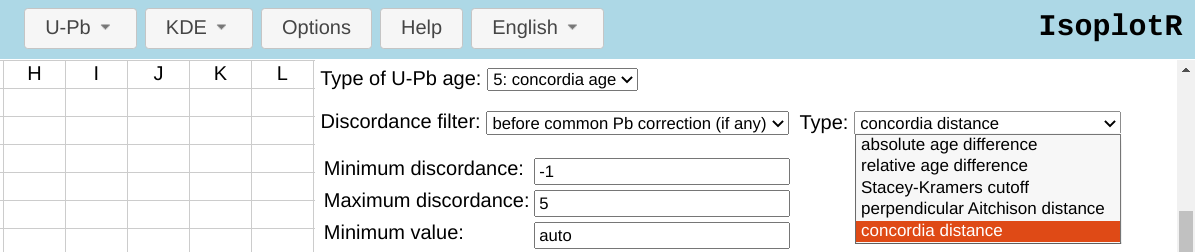
\includegraphics[width=12cm]{IsoplotR.png}
  \caption{The new discordance filters can be accessed from
    \texttt{IsoplotR}'s graphical user interface, shown here under its
    kernel density estimation function.}
  \label{fig:IsoplotR}
\end{figure}

To access the same functionality from the command line requires
installation of \texttt{IsoplotR} from the Comprehensive R Archive
Network (CRAN):

\begin{verbatim}
install.packages('IsoplotR')
\end{verbatim}

\noindent Once installed, the package must be added to the working
environment:

\begin{verbatim}
library(IsoplotR)
\end{verbatim}

\noindent Loading the test data into memory:

\begin{verbatim}
UPb <- read.data('data.csv',method='U-Pb',format=2)
\end{verbatim}

\noindent The discordance can then be calculated using
\texttt{IsoplotR}'s \texttt{discfilter} function. For example, to
compute the relative age discordance ($d_r$):

\begin{verbatim}
tr <- age(UPb,discordance=discfilter(option='r'))
\end{verbatim}

\noindent which produces a ${70,869}\times{9}$ table whose first eight
columns list the \textsuperscript{207}Pb/\textsuperscript{235}U,
\textsuperscript{206}Pb/\textsuperscript{238}U,
\textsuperscript{207}Pb/\textsuperscript{206}Pb and concordia ages and
their uncertainties, and whose ninth column lists the relative age
discordance as percentages. Similarly, to compute the concordia
distance ($d_c$):

\begin{verbatim}
tc <- age(UPb,discordance=discfilter(option='c'))
\end{verbatim}

\noindent Plotting a KDE of the single grain concordia ages that pass
the perpendicular Aitchison filter with ${-2}<{d_a}<{6}$:

\begin{verbatim}
df <- discfilter(option='c',cutoff=c(-2,6))
kde(UPb,type=5,cutoff.disc=df)
\end{verbatim}

\noindent Apply a Stacey-Kramers common Pb-correction to the data
after applying a Stacey-Kramers discordance filter with
${0}<{d_{sk}}<{0.96}$:

\begin{verbatim}
df <- discfilter(option='sk',cutoff=c(0,0.96))
kde(UPb,common.Pb=3,cutoff.disc=df)
\end{verbatim}

\noindent If the dataset includes \textsuperscript{204}Pb (which is
not the case for the test data), then we can also apply a discordance
filter \textit{after} the common Pb correction. For example:

\begin{verbatim}
df <- discfilter(option='r',before=FALSE,cutoff=c(-5,15))
kde(UPb,common.Pb=3,type=4,cutoff.76=1200,cutoff.disc=df)
\end{verbatim}

\noindent where \verb|option='r'| triggers the relative age filter
($d_r$), \texttt{common.Pb=3} applies a Stacey-Kramers type common Pb
correction, \texttt{type=4} uses the
\textsuperscript{206}Pb/\textsuperscript{238}U-age for young grains
and the \textsuperscript{207}Pb/\textsuperscript{206}Pb-age for old
ones, and \texttt{cutoff.76} marks the age (in Ma) at which to switch
from the \textsuperscript{206}Pb/\textsuperscript{238}U to the
\textsuperscript{207}Pb/\textsuperscript{206}Pb method. Further
information about these functions can be obtained from the built-in
documentation:

\begin{verbatim}
?IsoplotR
?discfilter
?kde
\end{verbatim}

\noindent Note that the examples shown here may take a few minutes to
complete due to the large size of the test dataset.


\section*{Acknowledgements}
  The writing of this paper was triggered by a stimulating email
  conversation with Chris Spencer and Steve Puetz.  The test data were
  compiled by Simon Bodorkos of Geoscience Australia, and the paper
  benefitted from careful reviews by Ping Wang and Keith Sircombe,
  with additional feedback from Chuck Magee.  This research was
  supported by NERC standard grant \#NE/T001518/1 (`Beyond Isoplot').

\begin{thebibliography}{14}
\providecommand{\natexlab}[1]{#1}
\providecommand{\url}[1]{{\tt #1}}
\providecommand{\urlprefix}{URL }
\expandafter\ifx\csname urlstyle\endcsname\relax
  \providecommand{\doi}[1]{https://doi.org/\discretionary{}{}{}#1}\else
  \providecommand{\doi}{https://doi.org/\discretionary{}{}{}\begingroup
  \urlstyle{rm}\Url}\fi

\bibitem[{Aitchison(1986)}]{aitchison1986}
Aitchison, J.: The statistical analysis of compositional data, London, Chapman
  and Hall, 1986.

\bibitem[{Cohen(1992)}]{cohen1992}
Cohen, J.: A power primer., Psychological bulletin, 112, 155, 1992.

\bibitem[{Gehrels(2011)}]{gehrels2011}
Gehrels, G.: {Detrital zircon U-Pb geochronology: Current methods and new
  opportunities}, in: Tectonics of sedimentary basins: Recent advances, edited
  by Busby, C. and Azor, A., chap.~2, pp. 45--62, Wiley Online Library, 2011.

\bibitem[{{Ludwig}(1998)}]{ludwig1998}
{Ludwig}, K.~R.: {On the treatment of concordant uranium-lead ages}, Geochimica
  et Cosmochimica Acta, 62, 665--676, \doi{10.1016/S0016-7037(98)00059-3},
  1998.

\bibitem[{{McIntyre} et~al.(1966){McIntyre}, {Brooks}, {Compston}, and
  {Turek}}]{mcintyre1966}
{McIntyre}, G.~A., {Brooks}, C., {Compston}, W., and {Turek}, A.: {The
  Statistical Assessment of Rb-Sr Isochrons}, Journal of Geophysical Research,
  71, 5459--5468, 1966.

\bibitem[{{Nemchin} and {Cawood}(2005)}]{nemchin2005}
{Nemchin}, A.~A. and {Cawood}, P.~A.: {Discordance of the U--Pb system in
  detrital zircons: Implication for provenance studies of sedimentary rocks},
  Sedimentary Geology, 182, 143--162, \doi{10.1016/j.sedgeo.2005.07.011}, 2005.

\bibitem[{Pawlowsky-Glahn et~al.(2015)Pawlowsky-Glahn, Egozcue, and
  Tolosana-Delgado}]{pawlowsky2015}
Pawlowsky-Glahn, V., Egozcue, J.~J., and Tolosana-Delgado, R.: Modeling and
  analysis of compositional data, John Wiley \& Sons, 2015.

\bibitem[{Puetz et~al.(2018)Puetz, Ganade, Zimmermann, and
  Borchardt}]{puetz2018}
Puetz, S.~J., Ganade, C.~E., Zimmermann, U., and Borchardt, G.: {Statistical
  analyses of global U-Pb database 2017}, Geoscience Frontiers, 9, 121--145,
  2018.

\bibitem[{Schoene(2014)}]{schoene2014}
Schoene, B.: U--Th--Pb Geochronology, Treatise on geochemistry, 4, 341--378,
  2014.

\bibitem[{Spencer et~al.(2016)Spencer, Kirkland, and Taylor}]{spencer2016}
Spencer, C.~J., Kirkland, C.~L., and Taylor, R.~J.: {Strategies towards
  statistically robust interpretations of in situ U--Pb zircon geochronology},
  Geoscience Frontiers, 7, 581--589, 2016.

\bibitem[{Stacey and Kramers(1975)}]{stacey1975}
Stacey, J. and Kramers, J.: Approximation of terrestrial lead isotope evolution
  by a two-stage model, Earth and Planetary Science Letters, 26, 207--221,
  1975.

\bibitem[{Vermeesch(2013)}]{vermeesch2013}
Vermeesch, P.: Multi-sample comparison of detrital age distributions, Chemical
  Geology, 341, 140--146, 2013.

\bibitem[{Vermeesch(2018)}]{vermeesch2018c}
Vermeesch, P.: {\texttt{IsoplotR}: a free and open toolbox for geochronology},
  Geoscience Frontiers, 9, 1479--1493, 2018.

\bibitem[{Zimmermann et~al.(2018)Zimmermann, Mark, Chew, and
  Voice}]{zimmermann2018}
Zimmermann, S., Mark, C., Chew, D., and Voice, P.~J.: {Maximising data and
  precision from detrital zircon U-Pb analysis by LA-ICPMS: The use of core-rim
  ages and the single-analysis concordia age}, Sedimentary geology, 375, 5--13,
  2018.

\end{thebibliography}

\end{document}
